\hypertarget{ux8af8ux8ad6}{%
\chapter{諸論}\label{ux8af8ux8ad6}}

\hypertarget{ux5f93ux6765ux306eux88fdux9020ux696d}{%
\section{従来の製造業}\label{ux5f93ux6765ux306eux88fdux9020ux696d}}

従来のモノづくり企業は垂直型経営が主流であった\cite{Suichoku}.垂直型経営とは設計,材料・部品の調達,製造,組立の一連のプロセスを自社でまかなう経営形態である.垂直型経営はノウハウを蓄積することが可能である,機密性を保てるなどのメリットがある.

\begin{center}\rule{0.5\linewidth}{0.5pt}\end{center}

\begin{itemize}
\tightlist
\item
  \textbf{\emph{垂直型経営についてもう少し述べる...}}
\end{itemize}

\begin{center}\rule{0.5\linewidth}{0.5pt}\end{center}

しかし,近年の製造業の顧客ニーズは多様化し,それにより製品品種の増加,製品ライフサイクルが短期化している.それによって,従来の垂直型経営における以下の課題点が浮き彫りになってきた.

\begin{center}\rule{0.5\linewidth}{0.5pt}\end{center}

\begin{itemize}
\tightlist
\item
  \textbf{\emph{顧客ニースの多様化の背景を書く...}}
\end{itemize}

\begin{center}\rule{0.5\linewidth}{0.5pt}\end{center}

\begin{itemize}
\tightlist
\item
  環境変化への対応

  \begin{itemize}
  \tightlist
  \item
    垂直型経営では自社で全ての固定ラインの生産システムを持っている.この生産システムでは近年の顧客ニーズの変化や需要変動に追従することができない.
  \end{itemize}
\item
  設備稼働率の低下

  \begin{itemize}
  \tightlist
  \item
    従来の生産システムは自社で全ての作業を行うことが多く,ピーク需要に合わせて生産能力を決定している.その結果として,設備稼働率が低下してしまう.そうすると固定費である生産設備費用が高くなり,高コスト・高アセットな製品となってしまう.
  \end{itemize}
\end{itemize}

上記の課題を解決する為に,クラウド技術の活用やIoT技術の活用に注目が集まっている.その中でも日本においてはシェアリング・エコノミーの考え方に基づいたモノづくりの分散化,製造リソースの共有に関する議論が盛んに行われている\cite{IVI}.

\hypertarget{ux30b7ux30a7ux30a2ux30eaux30f3ux30b0ux30a8ux30b3ux30ceux30dfux30fcux306eux767aux5c55}{%
\section{シェアリング・エコノミーの発展}\label{ux30b7ux30a7ux30a2ux30eaux30f3ux30b0ux30a8ux30b3ux30ceux30dfux30fcux306eux767aux5c55}}

近年IoT技術の発展を背景に,シェアリング・エコノミーが発展している.本節ではまずIoTについて説明を行い,その後,シェアリング・エコノミーについて述べる.

\hypertarget{iotux306eux767aux5c55}{%
\subsubsection{IoTの発展}\label{iotux306eux767aux5c55}}

近年,電子デバイスの低価格化,インターネットの発展によりIoT(Internet of
Things)の活用に注目が集まっている.IoTとは,ありとあらゆるものインターネット上に繋いでいく技術や概念である\cite{IoT2009}.IoTが普及すると,従来インターネットに接続されていなかったモノ(センサー機器,駆動装置(アクチュエータ)建物,車,電子機器などが)がインターネットを通じてサーバやクラウドサービスに接続され,相互に情報をやり取りすることができるようになる\cite{AWS-IoT}.

製造業においてもIoTを活用することで,製造業の効率化を狙う動きが活発化している.以下にその政策例を示す.

\begin{itemize}
\tightlist
\item
  Industrie 4.0\cite{Industrie4.0}

  \begin{itemize}
  \tightlist
  \item
    \textbf{\emph{Industrie 4.0について...}}
  \end{itemize}
\item
  Industrial Internet\cite{IIC}

  \begin{itemize}
  \tightlist
  \item
    \textbf{\emph{IICについて...}}
  \end{itemize}
\item
  \emph{中国}製造2025

  \begin{itemize}
  \tightlist
  \item
    \textbf{\emph{中国製造2025について書く...}}
  \end{itemize}
\end{itemize}

IoT技術を活用することで人やモノの位置,稼働状況などの情報を取得することができるようになる.さらにクラウドコンピューティング技術を活用することで,クラウド上にその情報を集約することが可能となる.そうするとことで,様々な人が情報にアクセスことが可能となり,実際の資源を共有し再利用をするシェアリング・エコノミーが促進されると考えらている\cite{Soumu-sharing}.

\hypertarget{ux30b7ux30a7ux30a2ux30eaux30f3ux30b0ux30a8ux30b3ux30ceux30dfux30fcux3068ux306f}{%
\subsubsection{シェアリングエコノミーとは}\label{ux30b7ux30a7ux30a2ux30eaux30f3ux30b0ux30a8ux30b3ux30ceux30dfux30fcux3068ux306f}}

シェアリング・エコノミーとは,典型的には個人が保有する遊休資産(スキルのような無形のものも含む)の貸出しを仲介,再利用するサービスであり,貸主は遊休資産の活用による収入,借主は所有することなく利用ができるというメリットがある\cite{Soumu-sharing}.前節のIoT技術の発展,情報の集約により,誰もが簡単に情報にアクセスすることが可能となることでシェアリング・サービスが急速に普及している.そのサービス例を以下に示す.

\begin{itemize}
\tightlist
\item
  メルカリ

  \begin{itemize}
  \tightlist
  \item
    \textbf{\emph{メルカリについて...}}
  \end{itemize}
\item
  Airbnb

  \begin{itemize}
  \tightlist
  \item
    \textbf{\emph{Airbnbについて...}}
  \end{itemize}
\end{itemize}

\hypertarget{ux88fdux9020ux696dux3078ux306eux5fdcux7528}{%
\subsubsection{製造業への応用}\label{ux88fdux9020ux696dux3078ux306eux5fdcux7528}}

製造業においてもシェアリング・エコノミーの考え方をとり入れることで,製造リソースをシェアリングすることで,従来の垂直統合の課題を克服し,企生産効率を高めることができる共生型モノづくりの実現を目指す動きが活発化している\cite{IVI}\cite{Hitachi-csmfg}.

\begin{center}\rule{0.5\linewidth}{0.5pt}\end{center}

\begin{itemize}
\tightlist
\item
  \textbf{\emph{IVIについてここで詳しく述べる...}}
\end{itemize}

\begin{center}\rule{0.5\linewidth}{0.5pt}\end{center}

\hypertarget{ux5171ux751fux578bux30e2ux30ceux3065ux304fux308a}{%
\section{共生型モノづくり}\label{ux5171ux751fux578bux30e2ux30ceux3065ux304fux308a}}

共生型モノづくりのコンセプトは,2013年に発表されたWuらの提言がしたCBDM(Cloud
Based Design and Manufacturing)が始めと考えられる\cite{WU2013}.

\hypertarget{cloud-based-design-and-manufacturing}{%
\subsection{Cloud Based Design and
Manufacturing}\label{cloud-based-design-and-manufacturing}}

クラウド技術を活用することで,製造業の活性化を図るのがCBDMの狙いである.具体的には以下のメリットが挙げられる.

\begin{itemize}
\tightlist
\item
  インターネットやクラウドサービスを活用することで,複数の人で製品を協調設計できる.
\item
  クラウド上で製造リソースを管理することで,必要に応じて分散された製造リソースを利用することができるようになる.
\end{itemize}

またCBDMの実現においては以下のシステム要件が必要とされている\cite{WU2015}.

\begin{itemize}
\tightlist
\item
  \textbf{\emph{システム要件を8個箇条書きで書く...}}
\end{itemize}

上記の要件はいずれも現在のIoT技術で実現が可能であり,共生型モノづくりに実現は現実味を帯びてきている.

以上の背景からFactory Of the
Futureにおいてリソースの相互融通に着目した生産形態であるクラウドソースドマニュファクチャリングの概念が提案された\cite{Factory2015}.

\hypertarget{ux30afux30e9ux30a6ux30c9ux30bdux30fcux30b9ux30c9ux30deux30cbux30e5ux30d5ux30a1ux30afux30c1ux30e3ux30eaux30f3ux30b0}{%
\subsection{クラウドソースドマニュファクチャリング}\label{ux30afux30e9ux30a6ux30c9ux30bdux30fcux30b9ux30c9ux30deux30cbux30e5ux30d5ux30a1ux30afux30c1ux30e3ux30eaux30f3ux30b0}}

Factory Of the
Futureにおいてクラウドソースドマニュファクチャリングとは,企業間で設備・材料・労働力・工法を融通し合う,共生に着目した生産形態であると記されている\cite{Factory2015}.以下にその概念図を示す.

\begin{itemize}
\tightlist
\item
  \textbf{\emph{Factory Of the Futureに載っている図を引用する...}}
\end{itemize}

クラウドソースドマニュファクチャリングを形成することで,従来のモノづくりの形態にはなかった以下のメリットがあると考える\cite{KATSUMURA2016}.

\begin{itemize}
\tightlist
\item
  \textbf{\emph{垂直統合にはないメリットを2つほど箇条書きで説明する...}}
\end{itemize}

このようにクラウドソースドマニュファクチャリングにおいては様々な独立した企業が参加し,リソースを相互に融通することで,従来より効率的な生産システムが実現する.

\begin{center}\rule{0.5\linewidth}{0.5pt}\end{center}

\begin{itemize}
\tightlist
\item
  リソース融通方法に他にどんなものがあるかを述べる.
\end{itemize}

\begin{center}\rule{0.5\linewidth}{0.5pt}\end{center}

\hypertarget{ux7814ux7a76ux76eeux7684}{%
\section{研究目的}\label{ux7814ux7a76ux76eeux7684}}

前節で述べたクラウドソースドマニュファクチャリングの共生の実現には,独立した企業が参加する状況下でも成り立つ企業間のリソース配分の仕組みが必要であるとされている\cite{Ghomi2019}.この問題に対して,目的の資源配分を自律的に実現する仕組みの設計を目標としたメカニズムデザインの観点,特に金銭取引を伴った資源配分を扱うオークションの知見が役立つと考える.実際に,メカニズムデザインの観点を考慮したリソース配分に関する研究は行われつつある\cite{THEKINEN2017}\cite{CHIDA2019}.しかし数は少なく,特に取引価格まで同時に決めることができるオークションに基づく研究は見当たらない.

そこで本研究では,クラウドソースドマニュファクチャリング実現に向けたリソース配分手法を提案する.特に買い手・売り手の双方が入札を行える組合せダブルオークションに基づくに着目し,オークションにおいて重要とされるパレート効率性を満たす手法,耐戦略性を満たす手法の2つ手法を提案する.そして計算機実験を行うことでそれぞれの手法の特性を解析を行うとともに,現実を想定したケーススタディを行い,両手法の位置付けを明らかにする.

\hypertarget{ux672cux8ad6ux6587ux306eux69cbux6210}{%
\section{本論文の構成}\label{ux672cux8ad6ux6587ux306eux69cbux6210}}

\begin{itemize}
\tightlist
\item
  \textbf{\emph{構成を書く...}}
\end{itemize}

\hypertarget{ux30afux30e9ux30a6ux30c9ux30bdux30fcux30b9ux30c9ux30deux30cbux30e5ux30d5ux30a1ux30afux30c1ux30e3ux30eaux30f3ux30b0ux306bux5bfeux3059ux308bux30aaux30fcux30afux30b7ux30e7ux30f3ux306eux9069ux7528}{%
\chapter{クラウドソースドマニュファクチャリングに対するオークションの適用}\label{ux30afux30e9ux30a6ux30c9ux30bdux30fcux30b9ux30c9ux30deux30cbux30e5ux30d5ux30a1ux30afux30c1ux30e3ux30eaux30f3ux30b0ux306bux5bfeux3059ux308bux30aaux30fcux30afux30b7ux30e7ux30f3ux306eux9069ux7528}}

\hypertarget{ux8af8ux8a00}{%
\section{諸言 }\label{ux8af8ux8a00}}

本章ではオークションを適用したクラウドソースドマニュファクチャリングモデルについて説明を行う.そしてオークションについての説明を行い,本研究で用いる組合せダブルオークションについて詳細な説明を行う.

\hypertarget{ux5bfeux8c61ux30e2ux30c7ux30eb}{%
\section{対象モデル}\label{ux5bfeux8c61ux30e2ux30c7ux30eb}}

本研究の対象であるクラウドソースドマニュファクチャリングに,オークションを適用したモデル図をFig.~\ref{fig:csmfg}に示す.

\begin{figure}[H]
\hypertarget{fig:csmfg}{%
\centering
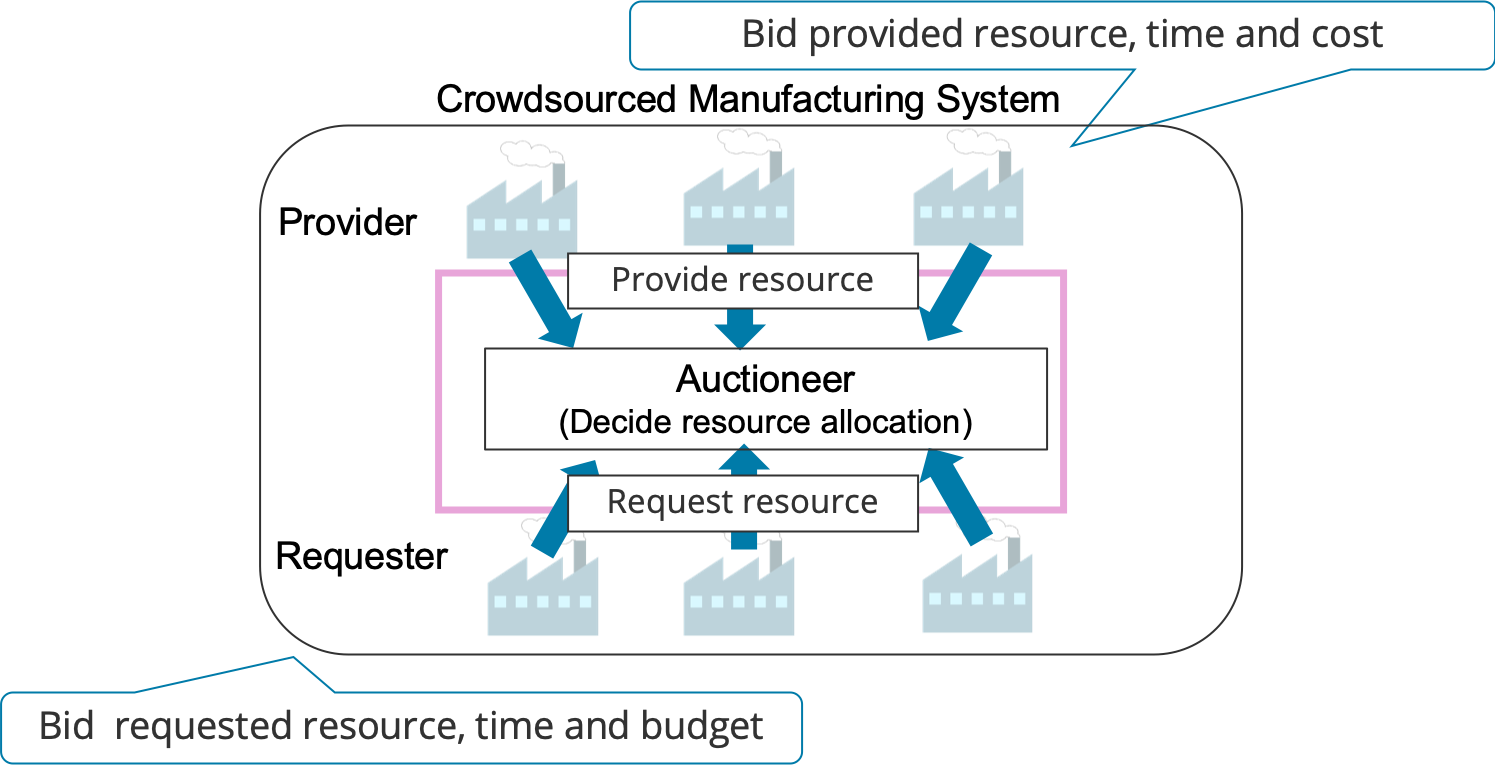
\includegraphics[width=0.4\textwidth,height=\textheight]{/Users/haradayoshiaki/Resarch/Paper/master-thesis/src/img/crowdsourced-manufacturing.png}
\caption{Crowedsourced Manufacturing}\label{fig:csmfg}
}
\end{figure}

リソースの提供側とリソースの要求側,そしてオークション主催者が存在する.それぞれの主体について説明する.

\begin{itemize}
\tightlist
\item
  リソース要求企業:要求するリソースの時間,予算を入札する.

  \begin{itemize}
  \tightlist
  \item
    予算はこの価格でリソースを使用すると利益が出ない価格とする.
  \end{itemize}
\item
  リソース提供企業:提供するリソースの時間,コストを入札する.

  \begin{itemize}
  \tightlist
  \item
    コストはこの価格でリソースの提供をしてしまうと利益が出ない値とする.
  \end{itemize}
\item
  オークション主催者:リソース提供・要求企業の入札を元にリソースの配分と,取引価格を決定する.

  \begin{itemize}
  \tightlist
  \item
    本研究においてはオークション主催者の利益は考慮しないものとする.
  \end{itemize}
\end{itemize}

\hypertarget{ux30aaux30fcux30afux30b7ux30e7ux30f3}{%
\section{オークション}\label{ux30aaux30fcux30afux30b7ux30e7ux30f3}}

本節ではオークションに関する一般的な説明を行った上で,本研究で行う組合せダブルオークションについて説明する.

\hypertarget{ux30aaux30fcux30afux30b7ux30e7ux30f3ux3068ux306f}{%
\subsection{オークションとは}\label{ux30aaux30fcux30afux30b7ux30e7ux30f3ux3068ux306f}}

オークションは,分散化された意思決定下において,財の配分と取引価格を決めるルールのことを指す.近年周波数帯オークション,ネット広告オークションでの成功から更に注目が集まっている.

オークションの説明に使用される用語を以下に示す.

\begin{itemize}
\tightlist
\item
  財:オークションにおいて取引される資源のこと.
\item
  入札:財に対する評価値を表明すること.

  \begin{itemize}
  \tightlist
  \item
    この値を入札値と呼ぶ.
  \end{itemize}
\item
  準線形環境:金銭と効用(利益)が交換可能な環境のこと.

  \begin{itemize}
  \tightlist
  \item
    オークションではほどんどの場合で準線形環境を仮定する.
  \end{itemize}
\item
  買い手:金銭を払って財を入手することで利益を得たい主体のこと.

  \begin{itemize}
  \tightlist
  \item
    買い手の利益は財を入手するのに必要だった価格と評価値の差である.

    \begin{itemize}
    \tightlist
    \item
      例.評価値1000円の財を500円で買った買い手の利益は500円となる.
    \end{itemize}
  \end{itemize}
\item
  売り手:財を売って金銭を得ることで利益を得たい主体のこと.

  \begin{itemize}
  \tightlist
  \item
    売り手の利益は実際に受け取った報酬と評価値の差である.

    \begin{itemize}
    \tightlist
    \item
      例.評価値500円の財を1000円で売った売り手の利益は500円となる.
    \end{itemize}
  \end{itemize}
\item
  真の評価値:その値で財の取引を行うと,利益が0となる値のこと.
\item
  オークション主催者:ある目的を達成するために入札を元に財の配分と価格を決める主体のこと.

  \begin{itemize}
  \tightlist
  \item
    オークションの目的は参加者の効用の合計(社会的余剰)の最大,つまり総利益の最大となることが多い.
  \end{itemize}
\end{itemize}

\hypertarget{ux30aaux30fcux30afux30b7ux30e7ux30f3ux306eux8ca1ux306bux95a2ux3059ux308bux5206ux985e}{%
\subsection{オークションの財に関する分類}\label{ux30aaux30fcux30afux30b7ux30e7ux30f3ux306eux8ca1ux306bux95a2ux3059ux308bux5206ux985e}}

まずオークションに掛けられる財の種類による分類を説明する.

\hypertarget{ux5358ux4e00ux8ca1ux30aaux30fcux30afux30b7ux30e7ux30f3}{%
\subsubsection{単一財オークション}\label{ux5358ux4e00ux8ca1ux30aaux30fcux30afux30b7ux30e7ux30f3}}

オークションにかけられる財が1つであるオークションのことを単一財オークションと言う.

\hypertarget{ux8907ux6570ux8ca1ux30aaux30fcux30afux30b7ux30e7ux30f3}{%
\subsubsection{複数財オークション}\label{ux8907ux6570ux8ca1ux30aaux30fcux30afux30b7ux30e7ux30f3}}

オークションにかけられる財が複数財であるオークションのことを複数財オークションと言う.その中でもさらに複数ユニットオークションと組合せオークションの2つに分類される.

\hypertarget{ux8907ux6570ux30e6ux30cbux30c3ux30c8ux30aaux30fcux30afux30b7ux30e7ux30f3}{%
\paragraph{複数ユニットオークション}\label{ux8907ux6570ux30e6ux30cbux30c3ux30c8ux30aaux30fcux30afux30b7ux30e7ux30f3}}

同じ種類の財が複数単位かけられるオークションを複数ユニットオークションと言う.

\hypertarget{ux7d44ux5408ux305bux30aaux30fcux30afux30b7ux30e7ux30f3}{%
\paragraph{組合せオークション}\label{ux7d44ux5408ux305bux30aaux30fcux30afux30b7ux30e7ux30f3}}

複数種類の財が複数単位オークションにかけられ,入手できる組合せによって財の価値が変わるオークションを組合せオークションと言う.組合せオークションでは財の組合せに対して入札が可能である.組合せオークションでは,財同士の価値の間に依存関係がある場合が存在する.例えば,メモリとパソコンのように,メモリだけでは無価値で,またメモリが少ないPCが使い勝手が悪いと言うように,同時に所有できると価値が高まるなどの関係である.

\hypertarget{ux30aaux30fcux30afux30b7ux30e7ux30f3ux306eux5165ux672dux306bux95a2ux3059ux308bux5206ux985e}{%
\subsection{オークションの入札に関する分類}\label{ux30aaux30fcux30afux30b7ux30e7ux30f3ux306eux5165ux672dux306bux95a2ux3059ux308bux5206ux985e}}

次にオークションの入札を誰が行うかに着目した分類の説明を行う.

\hypertarget{ux30b7ux30f3ux30b0ux30ebux30aaux30fcux30afux30b7ux30e7ux30f3ux30b7ux30f3ux30b0ux30ebux30b5ux30a4ux30c9ux30aaux30fcux30afux30b7ux30e7ux30f3}{%
\subsubsection{シングルオークション(シングルサイドオークション)}\label{ux30b7ux30f3ux30b0ux30ebux30aaux30fcux30afux30b7ux30e7ux30f3ux30b7ux30f3ux30b0ux30ebux30b5ux30a4ux30c9ux30aaux30fcux30afux30b7ux30e7ux30f3}}

入札を行う主体が買い手または売り手の片方である場合をシングルサイドオークションと言う.シングルサイドオークションの場合,入札者がオークション主催者の役割を担うことが多い.また売り手のみが入札を行うオークションを特にリバースオークションと呼ぶ場合もある.

\hypertarget{ux30c0ux30d6ux30ebux30aaux30fcux30afux30b7ux30e7ux30f3ux30c0ux30d6ux30ebux30b5ux30a4ux30c9ux30aaux30fcux30afux30b7ux30e7ux30f3}{%
\subsubsection{ダブルオークション(ダブルサイドオークション)}\label{ux30c0ux30d6ux30ebux30aaux30fcux30afux30b7ux30e7ux30f3ux30c0ux30d6ux30ebux30b5ux30a4ux30c9ux30aaux30fcux30afux30b7ux30e7ux30f3}}

入札を行う主体が買い手,売り手の双方である場合をダブルサイドオークションと言う.

\hypertarget{ux30aaux30fcux30afux30b7ux30e7ux30f3ux306eux8a55ux4fa1ux6307ux6a19}{%
\subsection{オークションの評価指標}\label{ux30aaux30fcux30afux30b7ux30e7ux30f3ux306eux8a55ux4fa1ux6307ux6a19}}

本節ではオークションが満たすべきとされる性質を説明する.

\hypertarget{ux500bux4ebaux5408ux7406ux6027}{%
\subsubsection{個人合理性}\label{ux500bux4ebaux5408ux7406ux6027}}

オークションに参加することで損をする者がいない性質を個人合理性と言う.個人合理性を満たさないオークションはオークションに参加することで損をしてしまう可能性があるので,参加者を集めることが極めて困難になる.

\hypertarget{ux30d1ux30ecux30fcux30c8ux52b9ux7387ux6027}{%
\subsubsection{パレート効率性}\label{ux30d1ux30ecux30fcux30c8ux52b9ux7387ux6027}}

誰かの効用を下げることに,他の誰かの効用を高めることができない状態をパレート効率的であると言う.そのような状態を導くオークションのことをパレート効率性を満たすオークションと言う.例えば,総利益が最大化されいる状態はパレート効率な状態であり,ある誰かの利益を下げない限り他の誰かの利益を上げることはできない.

\hypertarget{ux8010ux6226ux7565ux6027}{%
\subsubsection{耐戦略性}\label{ux8010ux6226ux7565ux6027}}

正直に真の評価値を申告することが支配戦略であるオークションを耐戦略性を満たすオークショと言う.つまり耐戦略性を満たすオークションでは.財に対する真の評価値をそのまま申告することが自分の利益を最大化する為の支配戦略となる.この性質を満たさないオークションは以下2点の欠点がある.

\begin{itemize}
\tightlist
\item
  オークション主催者が目指したい結果を正しく導くことができない

  \begin{itemize}
  \tightlist
  \item
    オークション主催者は入札者の評価値を元に財の配分を決める.しかし耐戦略性を満たさないオークションはその評価値が真の値とは限らず,導いた結果が本来の目的を達成できているかがわからない.
  \end{itemize}
\item
  入札者にとって使いづらいオークションになる

  \begin{itemize}
  \tightlist
  \item
    耐戦略性を満たさないオークションの場合正直な評価値の申告が支配戦略でないので,どのような評価値で入札するべきかを考える必要がある.
  \end{itemize}
\end{itemize}

\hypertarget{ux4ee3ux8868ux7684ux306aux30aaux30fcux30afux30b7ux30e7ux30f3ux306eux4f8b}{%
\subsection{代表的なオークションの例}\label{ux4ee3ux8868ux7684ux306aux30aaux30fcux30afux30b7ux30e7ux30f3ux306eux4f8b}}

本節では代表的なオークションについて説明する.

\hypertarget{ux30d5ux30a1ux30fcux30b9ux30c8ux30d7ux30e9ux30a4ux30b9ux30aaux30fcux30afux30b7ux30e7ux30f3}{%
\subsubsection{ファーストプライスオークション}\label{ux30d5ux30a1ux30fcux30b9ux30c8ux30d7ux30e9ux30a4ux30b9ux30aaux30fcux30afux30b7ux30e7ux30f3}}

\begin{center}\rule{0.5\linewidth}{0.5pt}\end{center}

\begin{itemize}
\tightlist
\item
  ファーストプライスオークションについて少し述べる
\end{itemize}

\begin{center}\rule{0.5\linewidth}{0.5pt}\end{center}

ファーストプライスオークションは以下の特徴を持つ.

\begin{itemize}
\tightlist
\item
  ルール

  \begin{itemize}
  \tightlist
  \item
    財に対する入札を一度だけ行う.

    \begin{itemize}
    \tightlist
    \item
      入札値はオークション主催者にしか公開されない
    \end{itemize}
  \item
    一番入札値が高い入札者がその入札値でその財を得ることができる(リバースオークションの場合は一番低い入札値の入札者が売ることができる)
  \end{itemize}
\item
  分類

  \begin{itemize}
  \tightlist
  \item
    単一財オークション
  \item
    シングルサイドオークション
  \end{itemize}
\item
  性質

  \begin{itemize}
  \tightlist
  \item
    個人合理性○
  \item
    パレート効率性×
  \item
    耐戦略性×
  \end{itemize}
\end{itemize}

ファーストプライスオークションは入札値がそのまま取引価格となるので,財に対する真の評価値に利益を上乗せした値を入札値として申告することになる.このオークションはルールがシンプルであり,また自分の入札値で取引が行われることから透明性が求められるネット広告オークションに使用される.しかし耐戦略性を満たせず,支配戦略が存在しないので,入札戦略が複雑になるなどのデメリットが存在する.

\hypertarget{ux30bbux30abux30f3ux30c9ux30d7ux30e9ux30a4ux30b9ux30aaux30fcux30afux30b7ux30e7ux30f3}{%
\subsubsection{セカンドプライスオークション}\label{ux30bbux30abux30f3ux30c9ux30d7ux30e9ux30a4ux30b9ux30aaux30fcux30afux30b7ux30e7ux30f3}}

\begin{center}\rule{0.5\linewidth}{0.5pt}\end{center}

\begin{itemize}
\tightlist
\item
  \textbf{\emph{セカンドプライスオークションについて少し述べる}}
\end{itemize}

\begin{center}\rule{0.5\linewidth}{0.5pt}\end{center}

セカンドプライスオークションは以下の特徴を持つ.

\begin{itemize}
\tightlist
\item
  ルール

  \begin{itemize}
  \tightlist
  \item
    財に対する入札を一度だけ行う

    \begin{itemize}
    \tightlist
    \item
      入札値はオークション主催者にしか公開されない
    \end{itemize}
  \item
    一番入札値が高い入札者が勝者となり,その次に高い入札者の入札値(二位の価格)でその財を得ることができる(リバースオークションの場合は一番低い入札値の入札者が,その次に低い入札値で売ることができる)

    \begin{itemize}
    \tightlist
    \item
      勝者が支払うこの価格は,このオークションの勝者になれる最小の価格(critical
      price)である
    \end{itemize}
  \end{itemize}
\item
  分類

  \begin{itemize}
  \tightlist
  \item
    単一財オークション
  \item
    シングルサイドオークション
  \end{itemize}
\item
  性質

  \begin{itemize}
  \tightlist
  \item
    個人合理性○
  \item
    パレート効率性○
  \item
    耐戦略性○
  \end{itemize}
\end{itemize}

セカンドプライスオークションは,二位の価格と財に対する真の評価値との差がオークションの勝者となった入札者の利益となる.このオークションは個人合理性・パレート効率性・耐戦略性を満たすことができる.現実の適用例としては,Yahooオークションなどが挙げられる.

\hypertarget{ux30b6ux30e9ux30d0ux65b9ux5f0f}{%
\subsubsection{ザラバ方式}\label{ux30b6ux30e9ux30d0ux65b9ux5f0f}}

\begin{itemize}
\tightlist
\item
  \textbf{\emph{ダブルオークションの例として証券取引のザラバ方式を取り上げる...}}
\end{itemize}

\hypertarget{ux7d44ux5408ux305bux30c0ux30d6ux30ebux30aaux30fcux30afux30b7ux30e7ux30f3}{%
\section{組合せダブルオークション}\label{ux7d44ux5408ux305bux30c0ux30d6ux30ebux30aaux30fcux30afux30b7ux30e7ux30f3}}

本節では提案する2種類の組合せダブルオークションに基づいたリソース配分手法の共通部分について説明をする.

その準備としてまず,組合せオークションの代表的なオークションであるVCG(Vickrey--Clarke--Groves
Auction)オークションのシングルサイドオークションの場合で説明をする.

\hypertarget{vcgux30aaux30fcux30afux30b7ux30e7ux30f3vickreyclarkegroves-auction}{%
\subsubsection{VCGオークション(Vickrey--Clarke--Groves
Auction)}\label{vcgux30aaux30fcux30afux30b7ux30e7ux30f3vickreyclarkegroves-auction}}

\begin{center}\rule{0.5\linewidth}{0.5pt}\end{center}

\begin{itemize}
\tightlist
\item
  \textbf{\emph{VCGオークショの説明を少し記述する}}
\end{itemize}

\begin{center}\rule{0.5\linewidth}{0.5pt}\end{center}

VCGオークションは以下の特徴を持つ.

\begin{itemize}
\tightlist
\item
  ルール

  \begin{itemize}
  \tightlist
  \item
    財に対する入札を一度だけ行う.

    \begin{itemize}
    \tightlist
    \item
      入札値はオークション主催者にしか公開されない.
    \end{itemize}
  \item
    財の配分(オークションの勝者)は目的が総利益最大である組合せ最適化問題を解くことで決定される.

    \begin{itemize}
    \tightlist
    \item
      この問題を勝者決定問題と呼ぶ.
    \end{itemize}
  \item
    オークションの勝者は勝者として留まれる最小の価格を支払う.

    \begin{itemize}
    \tightlist
    \item
      価格を決める式は後述する.
    \end{itemize}
  \end{itemize}
\item
  分類

  \begin{itemize}
  \tightlist
  \item
    組合せオークション
  \item
    シングルサイドオークション
  \end{itemize}
\item
  性質

  \begin{itemize}
  \tightlist
  \item
    個人合理性○
  \item
    パレート効率性○
  \item
    耐戦略性○
  \end{itemize}
\end{itemize}

VCGオークションはセカンドプライスオークションを一般化し,財の組合せに対する入札に対応したものである.理論的に優れた性質(個人合理性・パレート効率性・耐戦略性)を持つことからKing
of Mechanismsとも呼ばれる.

以下VCGオークション勝者決定問題,価格の決定方法にいついて詳しく説明し,その後で性質について詳しく説明する.ただし,買い手が入札の場合について説明する.

\hypertarget{ux52ddux8005ux6c7aux5b9aux554fux984cux306eux5b9aux5f0fux5316}{%
\paragraph{勝者決定問題の定式化}\label{ux52ddux8005ux6c7aux5b9aux554fux984cux306eux5b9aux5f0fux5316}}

VCGオークションの勝者を決める勝者決定問題は,組合せ最適化問題として定式化される.

定式化に用いた記号の定義は以下の通りである.

\begin{itemize}
\tightlist
\item
  \(j\): 買い手\(j \in \boldsymbol{J}\)
\item
  \(n\): 買い手\(j\)の入札\(n \in \boldsymbol{N}\)
\item
  \(f_{j,n}\):買い手\(j\)の\(n\)番目の入札の評価値
\item
  \(a_{j,n,r}\):買い手\(j\)の入札\(n\)に財\(r\)が含まれるとき1,含まれないとき0となる定数
\item
  \(r\):オークションにかけられる財\(r \in \boldsymbol{R}\)
\end{itemize}

\begin{align}
    {\rm max}\quad &\sum_{j\in\boldsymbol{J}}\sum_{n \in \boldsymbol{N}}f_{j,n} \times x_{j,n}  \label{eq:ca-obj}\\  
  {\rm s.t.} \quad &\sum_{j\in\boldsymbol{J}}\sum_{n\in\boldsymbol{N}} a_{j,n,r}\times x_{j,n}\leq 1 &(\forall r) \label{eq:ca-cap-sub}\\
                  &\sum_{n \in \boldsymbol{N}} x_{j,n}\leq 1            &(\forall j)\\
                  &x_{j,n} \in \{0,1\}          &(\forall j,\forall n) 
\end{align}

決定変数は\(x_{j,n}\)であり,この値が1のとき入札者\(j\)の入札\(n\)が勝者となり入札に含れる財が落札され,この値が0のときに入札者\(j\)の入札\(n\)のは敗者となる.\(\eqref{eq:ca-obj}\)は目的関数であり,入札値の合計の最大化を表す.\(\eqref{eq:ca-cap-sub}\)は財を落札できるのは高々1入札者であることを表す制約である.これは財の容量制約を表す.

\hypertarget{ux4fa1ux683cux306eux5f0f}{%
\paragraph{価格の式}\label{ux4fa1ux683cux306eux5f0f}}

\begin{itemize}
\tightlist
\item
  \textbf{\emph{VCGの価格決定式を書く..}}
\end{itemize}

\hypertarget{ux6027ux8ceaux306eux8a3cux660e}{%
\paragraph{性質の証明}\label{ux6027ux8ceaux306eux8a3cux660e}}

\begin{itemize}
\tightlist
\item
  \textbf{\emph{VCGが耐戦略性や個人合理性を示すことを説明する}}
\end{itemize}

従来の製造業における組合せオークションを応用した研究では,シングルサイドオークションが多く扱われてきた.しかし本研究のクラウドソースドマニュファクチャリングにおいては.リソース提供企業・リソース要求企業の双方の意思を反映させる為に,ダブルオークションを適用する.そうすることで,提供企業と要求企業の総利益が最大化される配分を求めることを可能とした.本研究で行う組合せダブルオークションは以下の特徴を持つ.

\begin{itemize}
\tightlist
\item
  入札者

  \begin{itemize}
  \tightlist
  \item
    提供側

    \begin{itemize}
    \tightlist
    \item
      複数ユニットオークション

      \begin{itemize}
      \tightlist
      \item
        リソース複数単位(複数時間)提供することが可能である.
      \end{itemize}
    \end{itemize}
  \item
    要求側

    \begin{itemize}
    \tightlist
    \item
      組合せオークション

      \begin{itemize}
      \tightlist
      \item
        全てのリソースが揃わないと製品を作るが出来ず,利益を得ることが出来ないからである.
      \end{itemize}
    \end{itemize}
  \end{itemize}
\item
  オークションの目的

  \begin{itemize}
  \tightlist
  \item
    提供企業,要求企業の総利益の最大化とする.
  \end{itemize}
\end{itemize}

\hypertarget{ux5171ux901aux306eux6d41ux308c}{%
\section{共通の流れ}\label{ux5171ux901aux306eux6d41ux308c}}

提案するリソース配分手法は大きく分けて2つの段階からなる.

\begin{enumerate}
\def\labelenumi{\arabic{enumi}.}
\tightlist
\item
  入札作成

  \begin{itemize}
  \tightlist
  \item
    リソース提供企業はオークション主催者に入札を行う

    \begin{itemize}
    \tightlist
    \item
      \textbf{\emph{文字を使ってどのような入札を作成するかを説明する...}}
    \end{itemize}
  \item
    リソース提供企業はオークション主催者に入札を行う

    \begin{itemize}
    \tightlist
    \item
      \textbf{\emph{文字を使ってどのような入札を作成するかを説明する...}}
    \end{itemize}
  \end{itemize}
\item
  オークション主催者はリソースの配分と,取引価格の決定する
\end{enumerate}

2の部分の具体的なアルゴリズムは次節以降で説明する.ここでは1について例を用いて説明する.

\begin{itemize}
\tightlist
\item
  \textbf{\emph{図を使い入札の例を示す...}}
\end{itemize}

\hypertarget{ux8a55ux4fa1ux6307ux6a19}{%
\subsection{評価指標}\label{ux8a55ux4fa1ux6307ux6a19}}

本研究で提案する2つの手法の評価指標について述べる.

\begin{itemize}
\tightlist
\item
  オークションの観点の評価指標

  \begin{itemize}
  \tightlist
  \item
    パレート効率性:総利益の値を評価する.
  \item
    耐戦略性

    \begin{itemize}
    \tightlist
    \item
      虚偽申告を行ったある1企業の利益を評価する.
    \end{itemize}
  \end{itemize}
\item
  クラウドソースドマニュファクチャリングの観点の評価指標

  \begin{itemize}
  \tightlist
  \item
    総提供企業利益

    \begin{itemize}
    \tightlist
    \item
      提供企業の利益の合計を評価する.
    \end{itemize}
  \item
    総要求企業利益

    \begin{itemize}
    \tightlist
    \item
      要求企業の利益の合計を評価する.
    \end{itemize}
  \item
    1提供企業利益
  \item
    1要求企業利益
  \item
    提供企業の稼働率の変化

    \begin{itemize}
    \tightlist
    \item
      リソースを提供する前と提供した後での稼働率の増加分について評価する.
    \end{itemize}
  \item
    勝者となった要求の割合

    \begin{itemize}
    \tightlist
    \item
      全要求企業の内,勝者となった要求の割合について評価する.
    \end{itemize}
  \end{itemize}
\end{itemize}

次章以降では,以上の評価指標を用いて手法I:パレート効率性を満たす手法・手法II:耐戦略性を満たす手法の特性を評価する.

\hypertarget{ux7d50ux8a00}{%
\section{結言}\label{ux7d50ux8a00}}

\hypertarget{ux624bux6cd5iux30d1ux30ecux30fcux30c8ux52b9ux7387ux6027ux3092ux6e80ux305fux3059ux624bux6cd5}{%
\chapter{手法I:パレート効率性を満たす手法}\label{ux624bux6cd5iux30d1ux30ecux30fcux30c8ux52b9ux7387ux6027ux3092ux6e80ux305fux3059ux624bux6cd5}}

\hypertarget{ux30a2ux30ebux30b4ux30eaux30baux30e0}{%
\section{アルゴリズム}\label{ux30a2ux30ebux30b4ux30eaux30baux30e0}}

\hypertarget{ux6982ux8981}{%
\subsection{概要}\label{ux6982ux8981}}

\hypertarget{ux5165ux672dux4f5cux6210}{%
\subsection{入札作成}\label{ux5165ux672dux4f5cux6210}}

\hypertarget{ux52ddux8005ux6c7aux5b9a}{%
\subsection{勝者決定}\label{ux52ddux8005ux6c7aux5b9a}}

\hypertarget{ux53d6ux5f15ux4fa1ux683cux6c7aux5b9a}{%
\subsection{取引価格決定}\label{ux53d6ux5f15ux4fa1ux683cux6c7aux5b9a}}

\hypertarget{ux7279ux6027ux8a55ux4fa1}{%
\section{特性評価}\label{ux7279ux6027ux8a55ux4fa1}}

\hypertarget{ux63d0ux4f9bux4f01ux696dux6570ux306eux5909ux66f4}{%
\subsection{提供企業数の変更}\label{ux63d0ux4f9bux4f01ux696dux6570ux306eux5909ux66f4}}

\hypertarget{ux8981ux6c42ux4f01ux696dux6570ux306eux5909ux66f4}{%
\subsection{要求企業数の変更}\label{ux8981ux6c42ux4f01ux696dux6570ux306eux5909ux66f4}}

\hypertarget{ux63d0ux4f9bux4f01ux696dux6570ux306eux5909ux66f4-1}{%
\subsection{提供企業数の変更}\label{ux63d0ux4f9bux4f01ux696dux6570ux306eux5909ux66f4-1}}

\hypertarget{ux63d0ux4f9bux4f01ux696dux306eux865aux507dux7533ux544aux7387ux306eux5909ux66f4}{%
\subsection{1提供企業の虚偽申告率の変更}\label{ux63d0ux4f9bux4f01ux696dux306eux865aux507dux7533ux544aux7387ux306eux5909ux66f4}}

\hypertarget{ux8981ux6c42ux4f01ux696dux306eux865aux507dux7533ux544aux7387ux306eux5909ux66f4}{%
\subsection{1要求企業の虚偽申告率の変更}\label{ux8981ux6c42ux4f01ux696dux306eux865aux507dux7533ux544aux7387ux306eux5909ux66f4}}

\hypertarget{ux865aux507dux7533ux544aux3092ux884cux3046ux63d0ux4f9bux4f01ux696dux6570ux306eux5909ux66f4}{%
\subsection{虚偽申告を行う提供企業数の変更}\label{ux865aux507dux7533ux544aux3092ux884cux3046ux63d0ux4f9bux4f01ux696dux6570ux306eux5909ux66f4}}

\hypertarget{ux865aux507dux7533ux544aux3092ux884cux3046ux8981ux6c42ux4f01ux696dux6570ux306eux5909ux66f4}{%
\subsection{虚偽申告を行う要求企業数の変更}\label{ux865aux507dux7533ux544aux3092ux884cux3046ux8981ux6c42ux4f01ux696dux6570ux306eux5909ux66f4}}

\hypertarget{ux63d0ux4f9bux5074ux304cux7533ux544aux3059ux308bux30b3ux30b9ux30c8ux306eux5e45ux306eux5909ux66f4}{%
\subsection{提供側が申告するコストの幅の変更}\label{ux63d0ux4f9bux5074ux304cux7533ux544aux3059ux308bux30b3ux30b9ux30c8ux306eux5e45ux306eux5909ux66f4}}

\hypertarget{ux8981ux6c42ux4f01ux696dux304cux7533ux544aux3059ux308bux4e88ux7b97ux306eux5e45ux306eux5909ux66f4}{%
\subsection{要求企業が申告する予算の幅の変更}\label{ux8981ux6c42ux4f01ux696dux304cux7533ux544aux3059ux308bux4e88ux7b97ux306eux5e45ux306eux5909ux66f4}}

\hypertarget{ux624bux6cd5iiux8010ux6226ux7565ux6027ux3092ux6e80ux305fux3059ux624bux6cd5}{%
\chapter{手法II:耐戦略性を満たす手法}\label{ux624bux6cd5iiux8010ux6226ux7565ux6027ux3092ux6e80ux305fux3059ux624bux6cd5}}

\hypertarget{ux30a2ux30ebux30b4ux30eaux30baux30e0-1}{%
\section{アルゴリズム}\label{ux30a2ux30ebux30b4ux30eaux30baux30e0-1}}

\hypertarget{ux6982ux8981-1}{%
\subsection{概要}\label{ux6982ux8981-1}}

\hypertarget{ux5165ux672dux4f5cux6210-1}{%
\subsection{入札作成}\label{ux5165ux672dux4f5cux6210-1}}

\hypertarget{ux63d0ux4f9bux5074ux306eux52ddux8005ux3068ux53d6ux5f15ux4fa1ux683cux6c7aux5b9a}{%
\subsection{提供側の勝者と取引価格決定}\label{ux63d0ux4f9bux5074ux306eux52ddux8005ux3068ux53d6ux5f15ux4fa1ux683cux6c7aux5b9a}}

\hypertarget{ux8981ux6c42ux5074ux306eux52ddux8005ux3068ux53d6ux5f15ux4fa1ux683cux6c7aux5b9a}{%
\subsection{要求側の勝者と取引価格決定}\label{ux8981ux6c42ux5074ux306eux52ddux8005ux3068ux53d6ux5f15ux4fa1ux683cux6c7aux5b9a}}

\hypertarget{ux7279ux6027ux8a55ux4fa1-1}{%
\section{特性評価}\label{ux7279ux6027ux8a55ux4fa1-1}}

\hypertarget{ux63d0ux4f9bux4f01ux696dux6570ux306eux5909ux66f4-2}{%
\subsection{提供企業数の変更}\label{ux63d0ux4f9bux4f01ux696dux6570ux306eux5909ux66f4-2}}

\hypertarget{ux8981ux6c42ux4f01ux696dux6570ux306eux5909ux66f4-1}{%
\subsection{要求企業数の変更}\label{ux8981ux6c42ux4f01ux696dux6570ux306eux5909ux66f4-1}}

\hypertarget{ux63d0ux4f9bux4f01ux696dux6570ux306eux5909ux66f4-3}{%
\subsection{提供企業数の変更}\label{ux63d0ux4f9bux4f01ux696dux6570ux306eux5909ux66f4-3}}

\hypertarget{ux63d0ux4f9bux4f01ux696dux306eux865aux507dux7533ux544aux7387ux306eux5909ux66f4-1}{%
\subsection{1提供企業の虚偽申告率の変更}\label{ux63d0ux4f9bux4f01ux696dux306eux865aux507dux7533ux544aux7387ux306eux5909ux66f4-1}}

\hypertarget{ux8981ux6c42ux4f01ux696dux306eux865aux507dux7533ux544aux7387ux306eux5909ux66f4-1}{%
\subsection{1要求企業の虚偽申告率の変更}\label{ux8981ux6c42ux4f01ux696dux306eux865aux507dux7533ux544aux7387ux306eux5909ux66f4-1}}

\hypertarget{ux865aux507dux7533ux544aux3092ux884cux3046ux63d0ux4f9bux4f01ux696dux6570ux306eux5909ux66f4-1}{%
\subsection{虚偽申告を行う提供企業数の変更}\label{ux865aux507dux7533ux544aux3092ux884cux3046ux63d0ux4f9bux4f01ux696dux6570ux306eux5909ux66f4-1}}

\hypertarget{ux865aux507dux7533ux544aux3092ux884cux3046ux8981ux6c42ux4f01ux696dux6570ux306eux5909ux66f4-1}{%
\subsection{虚偽申告を行う要求企業数の変更}\label{ux865aux507dux7533ux544aux3092ux884cux3046ux8981ux6c42ux4f01ux696dux6570ux306eux5909ux66f4-1}}

\hypertarget{ux63d0ux4f9bux5074ux304cux7533ux544aux3059ux308bux30b3ux30b9ux30c8ux306eux5e45ux306eux5909ux66f4-1}{%
\subsection{提供側が申告するコストの幅の変更}\label{ux63d0ux4f9bux5074ux304cux7533ux544aux3059ux308bux30b3ux30b9ux30c8ux306eux5e45ux306eux5909ux66f4-1}}

\hypertarget{ux8981ux6c42ux4f01ux696dux304cux7533ux544aux3059ux308bux4e88ux7b97ux306eux5e45ux306eux5909ux66f4-1}{%
\subsection{要求企業が申告する予算の幅の変更}\label{ux8981ux6c42ux4f01ux696dux304cux7533ux544aux3059ux308bux4e88ux7b97ux306eux5e45ux306eux5909ux66f4-1}}

\hypertarget{ux73feux5b9fux3092ux60f3ux5b9aux3057ux305fux30b1ux30fcux30b9ux30b9ux30bfux30c7ux30a3}{%
\chapter{現実を想定したケーススタディ}\label{ux73feux5b9fux3092ux60f3ux5b9aux3057ux305fux30b1ux30fcux30b9ux30b9ux30bfux30c7ux30a3}}

\hypertarget{ux7d50ux8ad6}{%
\chapter{結論}\label{ux7d50ux8ad6}}

\hypertarget{ux307eux3068ux3081}{%
\section{まとめ}\label{ux307eux3068ux3081}}

\hypertarget{ux4ecaux5f8cux306eux5c55ux671b}{%
\section{今後の展望}\label{ux4ecaux5f8cux306eux5c55ux671b}}
